
\pgfplotsset{
%        compat=newest,  % <-- does not work; don't know why
        compat=1.13,     % <-- works as expected
    }
  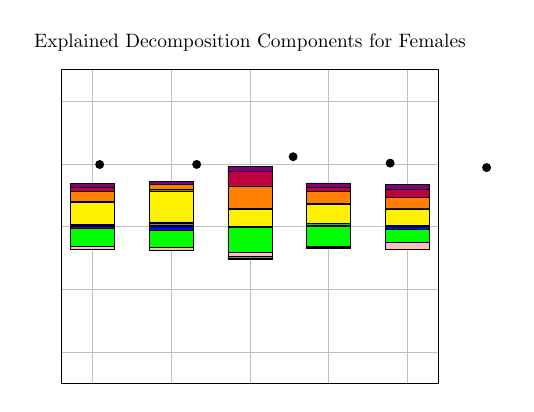
\begin{tikzpicture}[scale=0.7]
  %\node [align=center, font=\small, rotate=45,text width=2.15cm, inner sep=0.25cm] at (1, 1) {\textsc{year 1}};
  \begin{axis}[
    title={Explained Decomposition Components for Females},
    ybar stacked,
    ymax=0.5,
    ymin=-0.5,
    ymajorgrids = true,
    xmajorgrids = true,
    bar width=8mm,
    %xtick={1,2,3,4,5},
    %xticklabels={White, Black, Chinese, Asian, Mixed}
    symbolic x coords={non-White, Black, Chinese, Asian, Mixed},
    xtick=data,
    nodes near coords align={anchor=north},%Move values in bar
    every node near coord/.style={}
  ]
%married
\addplot [fill=blue] coordinates {({non-White},-0.0045978)({Black},-0.0123878)({Chinese},-0.0005473)({Asian},0.0004552)({Mixed},-0.0095788)};
%children
\addplot [fill=red] coordinates {({non-White},0.0029445)({Black},0.0043926)({Chinese},-0.0010838)({Asian},0.0032863)({Mixed},0.0007659)};
%UKyrs
\addplot [fill=green] coordinates {({non-White},-0.0572523)({Black},-0.0527464)({Chinese},-0.0786349)({Asian},-0.0618656)({Mixed},-0.0390382)};
%exp_ten
\addplot [fill=pink] coordinates {({non-White},-0.0094893)({Black},-0.0091958)({Chinese},-0.013803)({Asian},-0.0047749)({Mixed},-0.0224136)};
%public
\addplot [fill=gray] coordinates {({non-White},0.0000406)({Black},0.0047311)({Chinese},-0.0061328)({Asian},-0.0013175)({Mixed},-0.0021557)};
%u25
\addplot [fill=cyan] coordinates {({non-White},0.0050416)({Black},0.0060276)({Chinese},-0.0042301)({Asian},0.0064745)({Mixed},0.0030674)};
%region
\addplot [fill=yellow] coordinates {({non-White},0.0682828)({Black},0.0979206)({Chinese},0.0543122)({Asian},0.059861)({Mixed},0.0527352)};
%disability
\addplot [fill=black] coordinates {({non-White},0.000364)({Black},0.0001951)({Chinese},0.0014371)({Asian},0.0005247)({Mixed},-0.0002627)};
%pt
\addplot [fill=olive] coordinates {({non-White},0.0034646)({Black},0.0047695)({Chinese},0.0031673)({Asian},0.0030862)({Mixed},0.0033385)};
%educ
\addplot [fill=orange] coordinates {({non-White},0.0336574)({Black},0.0169901)({Chinese},0.070854)({Asian},0.0374063)({Mixed},0.0337004)};
%occup_ind
\addplot [fill=purple] coordinates {({non-White},0.0125542)({Black},-0.0021976)({Chinese},0.0474716)({Asian},0.0142189)({Mixed},0.0254938)};
%time
\addplot [fill=violet] coordinates {({non-White},0.0129348)({Black},0.0096944)({Chinese},0.0153423)({Asian},0.0141532)({Mixed},0.0144375)};

\addplot [only marks,mark=*,mark size=2pt,black,
         nodes near coords = \rotatebox{90}{{\pgfmathprintnumber[fixed zerofill,
                                    precision=2]{\pgfplotspointmeta}}},
        nodes near coords align={vertical},
        point meta=y,
        every node near coord/.append style={font=\small, yshift=0.25mm},] coordinates {({Mixed},-1)};
%\begin{comment}
%\end{comment}
%\filldraw[black] (0,0) circle (2pt) node[anchor=west] {Intersection point};
  \end{axis}
  
  \begin{axis}[
    nodes near coords align={anchor=north},%Move values in bar
    every node near coord/.style={},
    xtick=data,
    ymax=0.3,
    ymin=-0.3,
    xmax=0,
    xmin=5,
]
\pgfplotsset{ticks=none}
\addplot[only marks,mark=*,mark size=3pt,black,
         nodes near coords = \rotatebox{90}{{\pgfmathprintnumber[fixed zerofill,
                                    precision=2]{\pgfplotspointmeta}}},
        nodes near coords align={vertical},
        point meta=y,
        every node near coord/.append style={font=\small, yshift=0.25mm},
        ]  coordinates {
    (1,0.1) (2,-0.1) (3,1)
};
\end{axis}
\filldraw[black] (0.7,3.9756157) circle (2pt) node[anchor=west] {};
\filldraw[black] (2.46,3.9773538) circle (2pt) node[anchor=west] {};
\filldraw[black] (4.21,4.1170675) circle (2pt) node[anchor=west] {};
\filldraw[black] (5.97,4.0005588) circle (2pt) node[anchor=west] {};
\filldraw[black] (7.72,3.9206272) circle (2pt) node[anchor=west] {};
  \end{tikzpicture}
